\documentclass[12pt,a4paper,oneside]{report}
\usepackage[T1]{fontenc}
\usepackage[utf8]{inputenc}
\usepackage[sc]{mathpazo}
\usepackage[a4paper,left=3cm,right=2.5cm,top=3cm,bottom=3cm]{geometry}
\usepackage{graphicx,setspace,titlesec,fancyhdr,tabularx,booktabs,array,enumitem,caption,xcolor,ragged2e}
\usepackage[colorlinks=true,linkcolor=red,citecolor=red,urlcolor=black]{hyperref}
\titleformat{\chapter}[display]{\normalfont\bfseries\LARGE}{\Large\chaptertitlename\ \thechapter}{28pt}{\huge}
\titlespacing*{\chapter}{0pt}{60pt}{30pt}
\captionsetup{font=small,labelfont=bf}
\pagestyle{fancy}\fancyhf{}
\fancyhead[L]{\small\itshape\leftmark}\fancyfoot[C]{[\thepage]}
\renewcommand{\headrulewidth}{0.4pt}
\renewcommand{\chaptermark}[1]{\markboth{\chaptername\ \thechapter.\ #1}{}}
\fancypagestyle{plain}{\fancyhf{}\fancyfoot[C]{[\thepage]}\renewcommand{\headrulewidth}{0pt}}
\newcolumntype{L}[1]{>{\RaggedRight\arraybackslash}p{#1}}
\newcommand{\reporttitle}{Auracity: An AI Driven Civic Monitoring Platform}
\newcommand{\letterhead}{\noindent
\includegraphics[width=\textwidth]{letterhead.jpg}\par\vspace{1.2cm}}
\setlength{\parskip}{0.6em}\setlength{\parindent}{0pt}
\begin{document}

\begin{titlepage}\centering
{\LARGE\bfseries Auracity: An AI Driven\\[4pt] Civic Monitoring Platform\par}
\vspace{1.5cm}

\includegraphics[width=3.8cm]{logo.png}\par
\vspace{0.9cm}
\begin{tabular*}{0.92\textwidth}{@{\extracolsep{\fill}}lr}
\textit{By:-} & \textit{Enrollment No.}\\[2pt]
\textsc{Shivam Mishra} & IIT2024215\\
\textsc{Nitya Varma Datla} & IIT2024217\\
\textsc{Aadi Gosrani} & IIB2024005\\
\textsc{Adabala Sridhar} & IIT2024218\\
\textsc{Lucky Indrakant Raut} & IIB2024016\\
\textsc{Malhar Udmale} & IIB2024020\\
\end{tabular*}\par
\vspace{0.9cm}
{\small\itshape to the\par}\vspace{0.3cm}
{\large\textsc{Department of Information Technology}\par}\vspace{0.6cm}
{\large\textsc{Indian Institute of Information Technology,\\ Allahabad}\par}\vspace{0.8cm}
{\small November, 2026\par}
\end{titlepage}

\pagenumbering{roman}\setcounter{page}{1}
\setcounter{page}{1}\thispagestyle{plain}
\begin{center}{\small INDIAN INSTITUTE OF INFORMATION TECHNOLOGY, ALLAHABAD}\\[0.8cm]
\textbf{\reporttitle}\\[0.6cm] ABSTRACT\end{center}\vspace{0.3cm}
{\setstretch{1.9}Civic complaints in most Indian cities are still handled by hand. A citizen files a complaint, an office clerk reads it and forwards it to a department, and the citizen rarely hears anything again. Contractors are often paid without any clear proof that the repair was done. Auracity is our attempt to fix this chain from start to finish. A citizen takes one photo and drops a pin on the map. A vision model reads the photo, decides the type of issue and the department, and assigns it to a worker of that department. When the worker uploads a photo of the repair, the same model compares the before and after photos and gives a rating. Money moves from the city treasury to the worker only when this check passes, and every payment is written to a ledger that cannot be edited. This report describes how we arrived at the idea through the stages of design thinking, what we built, how we tested it and what each member contributed.\par}
\clearpage

{\setstretch{1.3}\listoffigures\clearpage\listoftables\clearpage}
\chapter*{List of Abbreviations}
\begin{center}\begin{tabular}{ll}
AI & Artificial Intelligence\\
API & Application Programming Interface\\
APK & Android Package\\
B2G & Business to Government\\
GPS & Global Positioning System\\
JSON & JavaScript Object Notation\\
RLS & Row Level Security\\
SQL & Structured Query Language\\
UI & User Interface\\
UPI & Unified Payments Interface\\
\end{tabular}\end{center}
\clearpage

\pagenumbering{arabic}
\setstretch{1.9}

\chapter{Introduction}
\section{Motivation}
Every city has potholes, broken street lights, garbage heaps and leaking pipes. The problem is usually not that nobody notices them. The problem is that the complaint gets lost somewhere between the citizen and the person who can fix it. Existing portals mostly stop at registering the complaint. They do not check whether the work was really done, and they do not show the citizen where the money went.

Auracity connects three kinds of users in one system. Citizens report issues and follow their status. Department workers, whom we call resolvers, receive jobs and get paid for verified repairs. City administrators watch the budget, review doubtful cases and manage contractors.

\section{Objectives and Scope}
The project was done as part of the Design Thinking and Innovation course. It has four objectives.
\begin{enumerate}
\item Understand why civic complaints fail today by talking to the people affected.
\item Design a flow that links the report, the repair, the proof and the payment.
\item Build a working prototype that uses a vision model to sort reports and to check repairs.
\item Prepare a business model that shows how the product can sustain itself.
\end{enumerate}
The prototype covers the complete flow for three roles. Real bank payouts and a city wide rollout are outside the scope of this report.

\section{Report Organization}
Chapter~\ref{ch:dt} describes the empathize, define and ideate stages. Chapter~\ref{ch:proto} explains the prototype and how it was implemented. Chapter~\ref{ch:test} gives the testing done and the results. Chapter~\ref{ch:biz} summarises the business model. Chapter~\ref{ch:end} lists the contribution of each member, the limitations, future work and the conclusion.

\chapter{Design Thinking Process}\label{ch:dt}
\section{Empathize}
We began by talking to people around us about the last time they complained about a civic problem. We spoke to students on campus, residents of nearby colonies in Prayagraj and a few shopkeepers near Jhalwa. We also looked at how existing municipal complaint portals and helpline numbers work. Three things came up again and again, as shown in Table~\ref{tab:empathy}.

\begin{table}[!htbp]\centering\setstretch{1.15}\small
\caption{Observations from the empathize stage.}\label{tab:empathy}
\begin{tabular}{L{6.2cm}L{8.3cm}}\toprule
\textbf{What people told us} & \textbf{What it means}\\\midrule
I complained twice about the same street light and nobody came. & Reports get lost. Staff sort complaints by hand and many reach the wrong department or wait in a queue.\\\addlinespace
The road was repaired last month and it is broken again. & Work is not verified. Contractors are paid without clear proof that the repair was done properly.\\\addlinespace
I have no idea what happened to my complaint. & Citizens see nothing. There is no live status and no record of spending, so trust in the system drops.\\\bottomrule
\end{tabular}\end{table}

We also noted that people are much more willing to take a photo than to fill a long form, and that they lose interest quickly if they get no response.

\section{Define}
From these observations we wrote one problem statement for the project.

\textbf{Citizens need a quick way to report civic issues and see them resolved, and city bodies need a way to pay only for work that is actually done, because the present process depends on manual sorting and unverified claims.}

We identified three users. The citizen wants to report in under a minute, see live status and feel that reporting is worth the effort. The resolver wants to see only the jobs given to them and to receive payment quickly after finishing the work. The city administrator wants no manual sorting, a clear view of budget and pending work, and proof behind every payment.

\section{Ideate}
We listed many ideas in our brainstorming sessions, such as a WhatsApp bot, a helpline with call recording and QR codes on every street pole. We compared them on effort for the citizen, cost for the city and how well they close the loop between report and payment. The idea we selected is a mobile app built around the four step chain in Table~\ref{tab:chain}.

\begin{table}[!htbp]\centering\setstretch{1.15}\small
\caption{The four step chain of Auracity.}\label{tab:chain}
\begin{tabular}{L{3cm}L{11.5cm}}\toprule
\textbf{Step} & \textbf{What happens}\\\midrule
1. Report & The citizen takes a photo and drops a pin on the map.\\\addlinespace
2. Classify & A vision model finds the issue type, the department, the severity and writes a short summary. The issue is assigned to a resolver of that department.\\\addlinespace
3. Resolve & The resolver fixes the issue and uploads an after photo from the same spot.\\\addlinespace
4. Audit and Pay & The model compares the before and after photos and rates the repair from 1 to 5. If the check passes, payment is released from the treasury to the wallet of the resolver.\\\bottomrule
\end{tabular}\end{table}

Along with this chain we decided on some supporting features. Citizens earn points for valid reports and can upvote issues, which raises the priority for the administrator. A City Mood feature shows the majority mood from citizen votes in the last two hours. A chat guide called AuraBot answers questions for new users.

\chapter{Prototype and Implementation}\label{ch:proto}
\section{What We Built}
We built a working mobile app for Android and iOS, a web version of the same system and the server side database. The mobile app is the main prototype and is the one we use for the demonstration. Its features are listed in Table~\ref{tab:features} and some screens are shown in Figure~\ref{fig:screens}.

\begin{table}[!htbp]\centering\setstretch{1.15}\small
\caption{Main features of the prototype.}\label{tab:features}
\begin{tabular}{L{3.8cm}L{10.7cm}}\toprule
\textbf{Feature} & \textbf{Description}\\\midrule
Live issue map & All issues appear as pins. Red means open or assigned, amber means under audit and green means fixed and verified.\\\addlinespace
Photo report & One photo, a map pin placed using GPS and an optional note.\\\addlinespace
Classification & The model returns the category, department, severity and a confidence value. Photos that are not civic issues are rejected.\\\addlinespace
Proof of Resolution & Before and after photos are compared. A reused photo or a photo of another place is rejected.\\\addlinespace
Safe payouts & Treasury to wallet transfer with a 2 percent platform fee, recorded in a ledger that only allows new entries.\\\addlinespace
Points and upvotes & 10 points for a valid report and 5 more when it is fixed. Upvotes raise priority.\\\addlinespace
City Mood & Majority mood from the latest vote of each citizen in the last two hours.\\\addlinespace
Admin dashboard & Budget, pending audits, priority list, department chart, contractor ratings and role management.\\\addlinespace
AuraBot & Chat guide that explains how to use the app.\\\bottomrule
\end{tabular}\end{table}

\begin{figure}[!htbp]\centering
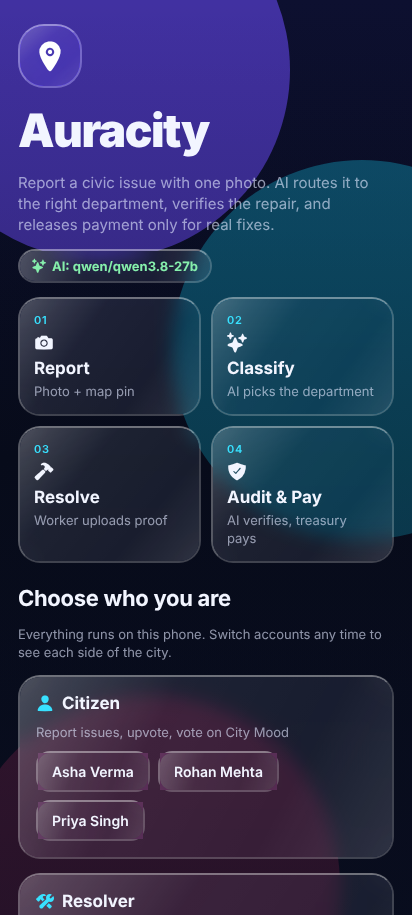
\includegraphics[width=0.24\textwidth]{m-login.png}\hfill
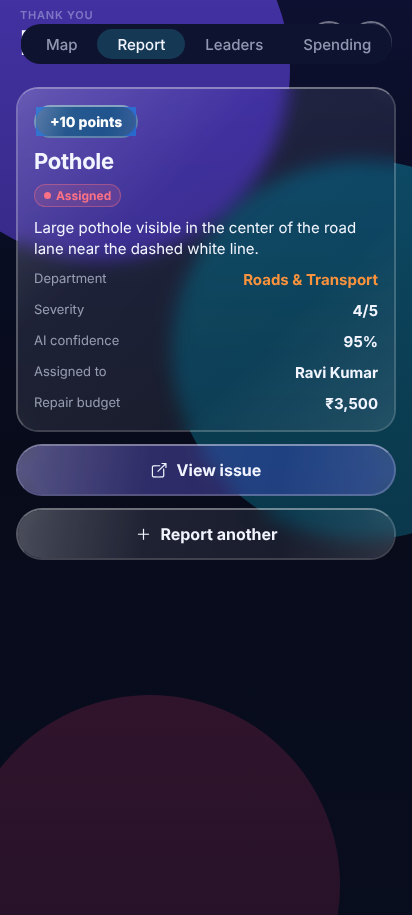
\includegraphics[width=0.24\textwidth]{m-reported.png}\hfill
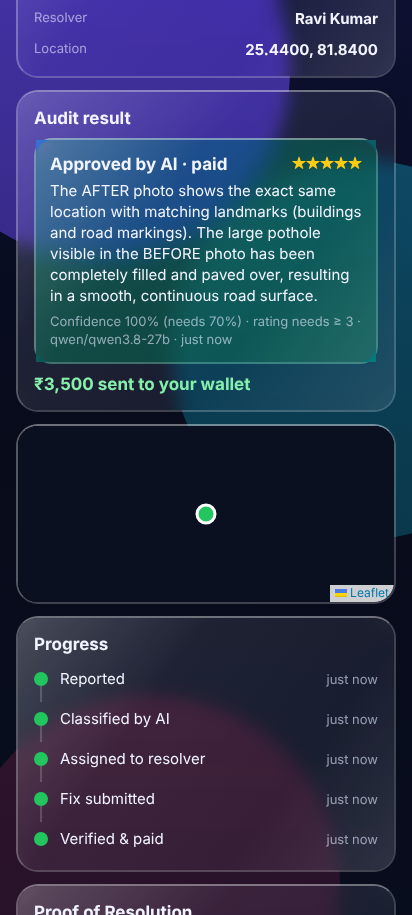
\includegraphics[width=0.24\textwidth]{m-audit.png}\hfill
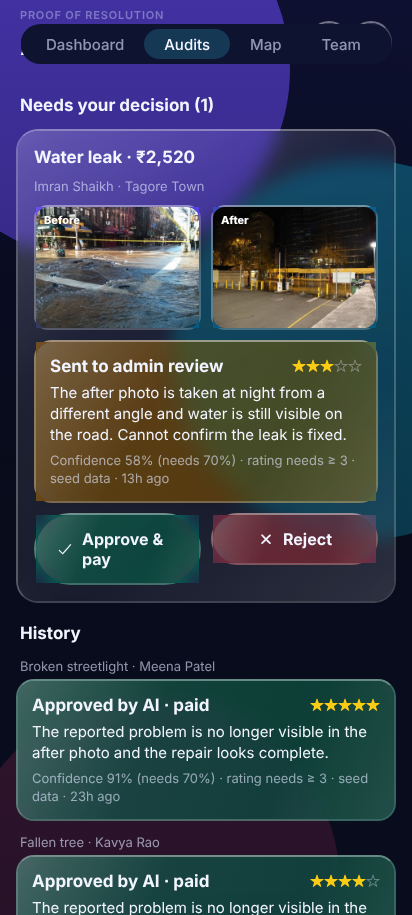
\includegraphics[width=0.24\textwidth]{m-audits.png}
\caption{Screens of the app. From left: sign in, result of a report after classification, audit result seen by the resolver, and audit review by the administrator.}\label{fig:screens}
\end{figure}

For the look of the app we followed the Liquid Glass style. Cards, buttons and the tab bar are translucent surfaces placed over a dark background with soft colour. On iPhones with iOS 26 the app uses the glass effect of the system itself. On Android, where this effect is not available, we draw a frosted surface with a light edge to get a similar feel.

\section{Technology Used}
The technology used in each layer is given in Table~\ref{tab:tech}.

\begin{table}[!htbp]\centering\setstretch{1.15}\small
\caption{Technology stack.}\label{tab:tech}
\begin{tabular}{L{2.6cm}L{5.4cm}L{6.2cm}}\toprule
\textbf{Layer} & \textbf{Technology} & \textbf{Purpose}\\\midrule
Mobile app & React Native with Expo, JavaScript & Android and iOS app from one code base\\\addlinespace
Web app & React, Vite, TypeScript & Browser version and admin dashboard\\\addlinespace
Maps & Leaflet with OpenStreetMap & Map and pins without a paid map key\\\addlinespace
AI & Groq API with the Qwen 3.8 vision model & Classification, repair audit and AuraBot\\\addlinespace
Backend & Supabase (PostgreSQL, Auth, Realtime, Storage) & Shared database, login, live updates and photos\\\addlinespace
Server logic & PL/pgSQL functions, triggers and edge functions & Payment engine, security rules, AI calls with a hidden key\\\addlinespace
Tools & Git, GitHub, Expo Application Services & Version control and Android build\\\bottomrule
\end{tabular}\end{table}

Our first plan, shown in the presentation, was to write the app in Flutter and to use the Llama 4 vision model. During development we moved to React Native because the team was more comfortable with JavaScript and it let us share logic with the web version. The Llama vision model was no longer offered on Groq when we started testing, so we changed to the Qwen vision model, which gave correct results in our tests.

\section{How the Pipeline Works}
When a citizen submits a report, the photo is compressed on the phone and sent to the vision model with a fixed instruction. The model must answer only in JSON with the fields we ask for. The app reads the department from the answer, calculates the repair budget from the base amount of that department and the severity, and gives the job to the resolver of that department who has the fewest open jobs.

When the resolver uploads the after photo, both photos are sent to the model with a stricter instruction that asks whether it is the same place and whether the problem is gone. The repair is approved if the model says it is genuine, the rating is 3 or more and the confidence is at least 70 percent. If the confidence is lower, the case goes to the administrator. Otherwise the job returns to the resolver.

Payment is done in one step. The treasury is reduced, the wallet is increased, the platform fee is taken and the ledger entries are written together. If any part fails, nothing is saved. In the database version this is a PL/pgSQL function that locks the treasury row, and normal users have no permission to call it directly.

\section{Security}
In the Supabase database we used Row Level Security and column level permissions. A citizen can insert a report but cannot set its status. Nobody can update the wallet, treasury or ledger tables from the app. All such changes go through database functions that first check the role of the caller. New accounts always start as citizens and only an administrator can make someone a resolver.

\section{Present Status}
The mobile app runs the full pipeline with the real AI model and keeps its data on the phone, which lets one phone show all three roles during a demonstration. The Supabase schema, the security rules, the payment function and the three edge functions are written and tested. The web app connects to Supabase when the project keys are provided. Connecting the mobile app to the shared database is the next step.

\chapter{Testing and Results}\label{ch:test}
\section{Test Cases}
We tested the complete flow several times with the real model. The main test cases and their results are given in Table~\ref{tab:tests}.

\begin{table}[!htbp]\centering\setstretch{1.15}\small
\caption{Test cases and results.}\label{tab:tests}
\begin{tabular}{L{4.6cm}L{3.4cm}L{6.2cm}}\toprule
\textbf{Test} & \textbf{Expected} & \textbf{Result}\\\midrule
Report a pothole photo with a short note & Sent to roads department & Passed. Category Pothole, severity 4 of 5, confidence 95 percent\\\addlinespace
Resolver uploads the same photo as proof & Rejected & Passed. The model reported that the after photo is identical to the before photo\\\addlinespace
Resolver uploads a real after photo & Approved and paid & Passed. Rating 5, amount added to wallet, payout and fee in ledger\\\addlinespace
After photo of a different problem & Rejected & Passed. The model said the pothole was not repaired\\\addlinespace
Low confidence audit & Sent to administrator & Passed. Administrator could approve or reject\\\addlinespace
Citizen tries to change points, treasury or ledger in the database & Blocked & Passed. Permission denied in every case\\\addlinespace
Edit or delete a ledger entry & Blocked & Passed. Ledger only accepts new entries\\\bottomrule
\end{tabular}\end{table}

\section{Problems Found and Fixed}
During testing we found and fixed some problems. The free plan of the AI service allows only a few image requests per minute, so we added an automatic wait and retry. The first map provider started asking for a key, so we changed to OpenStreetMap. On newer Android phones the keyboard was covering the text box, which we corrected.

\chapter{Business Model}\label{ch:biz}
\section{Overview}
Auracity is a business to government product. City bodies pay for it, citizens use it free and resolvers are paid through it. Other complaint portals stop at logging the complaint. Auracity links the report, the repair, the proof and the payment in one chain that can be audited. The main blocks of our business model canvas are summarised in Table~\ref{tab:bmc}.

\begin{table}[!htbp]\centering\setstretch{1.15}\small
\caption{Summary of the business model canvas.}\label{tab:bmc}
\begin{tabular}{L{3.6cm}L{10.9cm}}\toprule
\textbf{Block} & \textbf{Summary}\\\midrule
Customer segments & Municipal corporations and ward offices as paying customers, citizens and resolvers as users. Later, campuses and gated communities.\\\addlinespace
Value proposition & Fast reporting, automatic sorting, AI verified repairs and transparent spending.\\\addlinespace
Channels & Mobile app, admin dashboard, direct pilots with city bodies, QR codes in public places.\\\addlinespace
Revenue & Yearly subscription from city bodies, a small fee on each verified repair, setup fee and analytics.\\\addlinespace
Key resources & The app and database, the audit pipeline and the issue data collected over time.\\\addlinespace
Key partners & City departments, contractors, cloud and AI providers, payment gateways.\\\addlinespace
Costs & AI and cloud usage that grows with each report, team, onboarding and marketing.\\\bottomrule
\end{tabular}\end{table}

\section{Cost Control}
Each issue needs two AI calls, one to classify and one to audit. We keep this cost low by compressing photos before sending them and by using free plans during the pilot. Prices will be fixed after a pilot in one ward.

\chapter{Contributions and Conclusion}\label{ch:end}
\section{Individual Contributions}
The work was divided according to the interest and skill of each member. Everyone took part in the interviews, the brainstorming sessions and the testing. Table~\ref{tab:contrib} gives the main responsibility of each member.

\begin{table}[!htbp]\centering\setstretch{1.15}\small
\caption{Contribution of each member.}\label{tab:contrib}
\begin{tabular}{L{3.2cm}L{2.5cm}L{8.8cm}}\toprule
\textbf{Member} & \textbf{Roll number} & \textbf{Main work}\\\midrule
Adabala Sridhar & IIT2024218 & Led the development of the mobile app. Built the report, classify, resolve and audit flow, connected the AI model to the app, prepared the Android build and handled integration and bug fixing across the app.\\\addlinespace
Shivam Mishra & IIT2024215 & Database design in Supabase. Wrote the tables, the security policies and the payment and ledger functions, and tested them against misuse.\\\addlinespace
Nitya Varma Datla & IIT2024217 & AI part of the project. Wrote and tuned the instructions for classification and for the repair audit, compared models and decided the approval rule.\\\addlinespace
Aadi Gosrani & IIB2024005 & Web app and admin dashboard, including the budget view, audit review, contractor table and ledger screens.\\\addlinespace
Lucky Indrakant Raut & IIB2024016 & User interface design in the Liquid Glass style, map screen, City Mood, points and leaderboard, and the sample data used in the demonstration.\\\addlinespace
Malhar Udmale & IIB2024020 & User interviews and problem definition, business model canvas, presentation, test cases and documentation.\\\bottomrule
\end{tabular}\end{table}

\section{Limitations}
The mobile app stores data on the device, so two phones do not yet see the same issues. The free AI plan is slow when many audits are done together. The vision model can be wrong when the after photo is taken from a very different angle, which is why doubtful cases go to a human administrator. Wallet balances are numbers inside the system and are not yet linked to a bank or UPI.

\section{Future Work}
Our next steps are to connect the mobile app to the Supabase backend so that all users share live data, to add real payouts through a payment gateway, to support Hindi and other local languages, and to run a pilot in one ward to measure the accuracy of the audit and decide pricing.

\section{Conclusion}
Through this project we learnt to start from the user and not from the technology. The interviews showed us that the real gap is not in reporting but in what happens after the report. Auracity closes that gap by linking the report, the repair, the proof and the payment in one chain. The prototype shows that a vision model can sort complaints and check repairs well enough to be useful, as long as a human stays in the loop for doubtful cases. We believe that with a pilot and a shared backend this can become a practical tool for city bodies.

\renewcommand{\bibname}{References}
\begin{thebibliography}{9}\setstretch{1.3}
\addcontentsline{toc}{chapter}{References}
\bibitem{rn} Meta Platforms. \textit{React Native Documentation}. \url{https://reactnative.dev}
\bibitem{expo} Expo. \textit{Expo Documentation}. \url{https://docs.expo.dev}
\bibitem{supabase} Supabase. \textit{Supabase Documentation}. \url{https://supabase.com/docs}
\bibitem{groq} Groq. \textit{Groq API Documentation}. \url{https://console.groq.com/docs}
\bibitem{leaflet} Volodymyr Agafonkin. \textit{Leaflet, a JavaScript library for interactive maps}. \url{https://leafletjs.com}
\bibitem{osm} OpenStreetMap contributors. \textit{OpenStreetMap}. \url{https://www.openstreetmap.org}
\bibitem{bmg} Alexander Osterwalder and Yves Pigneur. \textit{Business Model Generation}. Wiley, 2010.
\bibitem{ov} Openverse. Source of the Creative Commons sample photographs used in the demonstration. \url{https://openverse.org}
\end{thebibliography}
\end{document}
